\documentclass[a4paper, 11pt]{book}
\usepackage[T1]{fontenc}
\usepackage[utf8]{inputenc}
\usepackage[french]{babel}
\usepackage[]{palatino}
\usepackage[]{graphicx}
    \setkeys{Gin}{width=0.95\linewidth}
    \graphicspath{./Captures}
\usepackage[]{float}
    \floatplacement{figure}{H}
    \floatplacement{table}{H}
\usepackage[table]{xcolor}
	\rowcolors{1}{white!95!black}{white}
\usepackage[]{hyperref}
    \hypersetup{
        colorlinks=true,
        linkcolor=blue,
        urlcolor=blue!50!purple,
    }
    \urlstyle{same}
\usepackage[]{array}
%\usepackage[margin=35mm]{geometry}
\usepackage[all, defaultlines=3]{nowidow}
%\usepackage[]{}
\title{Formation Apps.education}
\author{F.S.G.}
\date{Compilation du \today{}.}
\renewcommand{\baselinestretch}{1.25}
\setlength{\parskip}{0.5em}
\begin{document}
\begin{titlepage}
    \maketitle
\end{titlepage}

\chapter*{Introduction}
\addcontentsline{toc}{chapter}{Introduction}

Suite --ou en parallèle-- de la formation dispensée au collège, ce livret dont la vocation est de servir aussi bien de trame formative mais aussi de guide de référence au long terme puisqu'au fur et à mesure des révisions ce livret sera enrichi de nombreux chapitres consacrés aux applications indidividuelles présentes ou s'intégrant au bouquet de service offert sur apps.

Il est aussi possible de contribuer à l'élaboration du livre puisqu'il est présent sur un dépôt \emph{github} dont l'adresse figure à la fin de cet ouvrage. 

Où trouver de l'information ? C'est relativement simple, elle est disponible sur les salons du réseau social \textbf{tchap} dédiés à \emph{apps} : \url{https://matrix.to/#/#apps.education.fr:agent.education.tchap.gouv.fr} ouvert à toutes celles et ceux pouvant accéder au réseau.

Par choix, j'ai décidé d'articuler ce document de la manière suivante~:
\begin{itemize}
	\item cette introduction,
	\item la genèse et un court historique du projet,
	\item la connexion au service, que le compte soit déjà créé ou non,
	\item un survol sommaire des différents services logiciels proposé au sein du bouquet numérique,
	\item l'examen plus approfondi et précis des possibilités offertes par le nuage
	\item l'examen plus précis de chaque application au fur déjà présente
	\item viendront ensuite s'ajouter les examens plus précis des nouvelles applications ajoutées ...
	\item une table des contenus --chapitres, sections, fiches pratiques ...-- 
	\item les remerciements et informations légales
\end{itemize}

\paragraph*{Participation.}
Le choix qui a été fait est de privilégier des langages d'écritures textuels les plus purs possibles, excluant \emph{de facto\/} les documents compressés bureautiques classiques (.doc, .docx, .odt). 
Cependant, dans un esprit de bienveillance et d'accueil des bonnes volontés, si vous savez enregistrer vos documents en ``document plat XML'' --disponibles avec \emph{Office} de Microsoft et \emph{libreoffice} de la Document Foundation-- ou bien, que dans un effort de formation vous vous initiez à l'utilisation de langages très simples tels que \emph{Markdown}\footnote{%
Descriptif du langage : \url{https://fr.wikipedia.org/wiki/Markdown} ; Un descriptif des quelques balises de formatage \url{https://www.ionos.fr/digitalguide/sites-internet/developpement-web/markdown/} et une petite leçon sur ce langage \url{https://programminghistorian.org/fr/lecons/debuter-avec-markdown}
}


\section*{Révisions du document}
\begin{table}
	\centering
	\renewcommand{\arraystretch}{1.25}
	\begin{tabular}{| m{0.15\linewidth} | m{0.1\linewidth} | m{0.15\linewidth} | m{0.55\linewidth} |}
		\hline
		Date & n$^0$ de version & Auteur principal & Modifications apportées \cr
		\hline
		2022-06-15 & 0.01 & F.S.G. & Création du document (Markdown) \cr
		\hline
		2022-06-17 & 0.02 & F.S.G. & Passage Markdown $\rightarrow$ \LaTeX{} \newline Plan modifié \cr
		\hline
	\end{tabular}
\end{table}


\paragraph{Objectif} : Initier les collègues à l'utilisation du portail apps mis en place par notre ministère pour tous les agents qu'ils soient en académie ou en administration centrale. 

\chapter*{Un peu d'histoire}
\addcontentsline{toc}{chapter}{Un peu d'histoire}

\emph{Apps} est un projet initié en 2017 par les équipes du ministère (Bureau B1-1 de la direction du Numérique Éducatif) pour proposer aux agents un environnement numérique  moderne et répondant aux usages des utilisateurs, dans le cadre du projet SNP (Service Numériques Partagés). 
En effet la fragmentation des usages liée au nombre important des membres de l'éducation nationale --estimés dans le rapport à 1,2 millions d'agents dont environ 900~000 enseignants et 300~000 non-enseignants--, la diversité des métiers --une centaine répertoriés-- et par conséquent des usages rend difficile de proposer un outil unique avec un usage monolithique. 
Le choix d'un agréggateur de services permettant à chacun d'activer les services correspondant à ses usage a été alors préféré.

Ce projet a été ensuite récupéré par le bureau \og~Socle Numérique~\fg{} afin d'offrir aux agents des outils numériques de travail collaboratif mais toujours avec l'optique d'outils numérique, collaboratifs et accessibles sur le lieu de travail ou à l'extérieur, domicile compris.

Le service centralisateur, appelé ``La Boite'',  est situé ici : \url{https://portail.apps.education.fr}

Cette formation et son livret d'accompagnement s'organisent suivant le plan suivant~:
\begin{itemize}
    \item Création du compte
    \item Présentation des services
    \item Présentation plus détaillée du \emph{cloud\/}.
\end{itemize}

\chapter*{Créer son compte}
\addcontentsline{toc}{chapter}{Créer son compte}

La première chose à faire est de se connecter au site du portail qui est situé à \url{https://portail.apps.education.fr} comme le montre la capture d'écran suivante~:
\begin{figure}
    \centering
    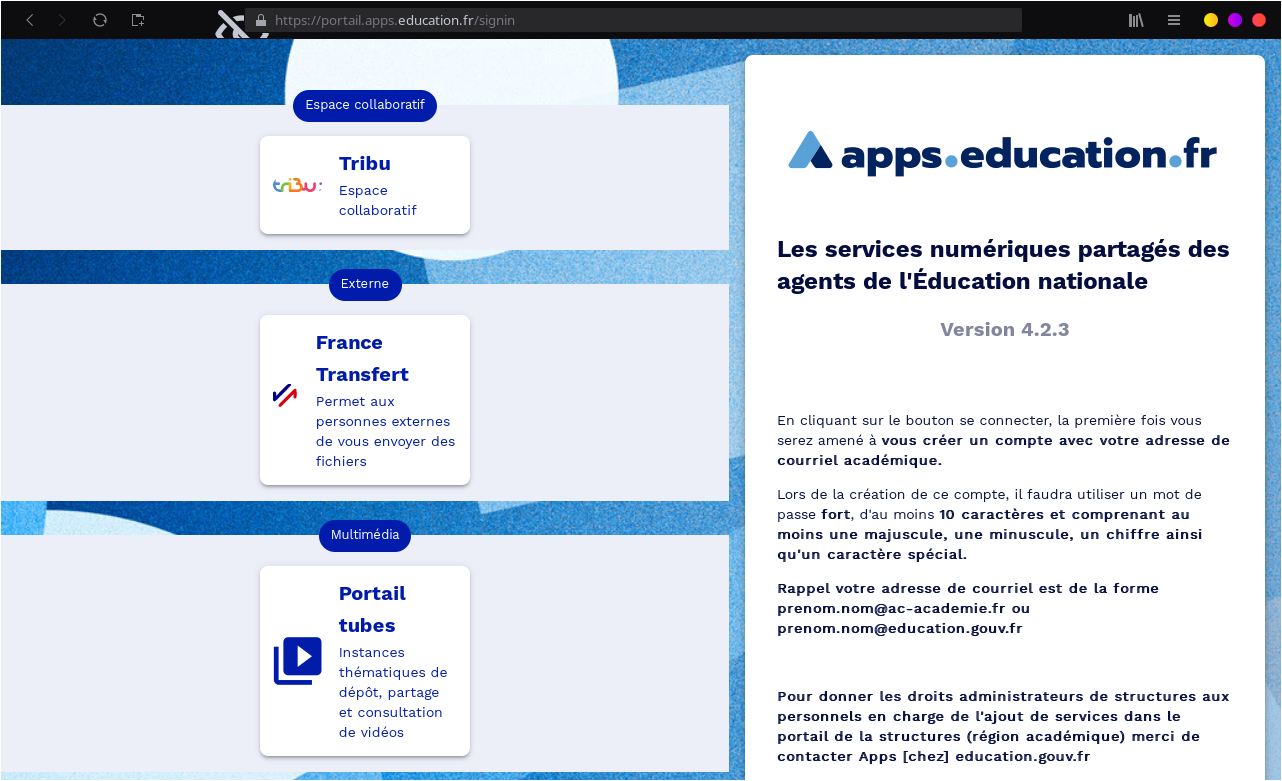
\includegraphics{Captures/portail.site.web.png}
\end{figure}

\chapter*{Découvrir les différents services}
\addcontentsline{toc}{chapter}{Découvrir les différents services}

bla bla bla

\chapter*{Utiliser le nuage}
\addcontentsline{toc}{chapter}{Utiliser le nuage}

bla lbla

\section*{L'interface Web}
\addcontentsline{toc}{section}{L'interface web}

bla lbla

\section*{Le client NextCloud}
\addcontentsline{toc}{section}{Le client nextcloud}

bla lbla

\section*{Transfert de données}
\addcontentsline{toc}{section}{Transfert de données}

bla lbla

\subsection*{Monter un ou plusieurs fichiers}
\addcontentsline{toc}{subsection}{Monter un ou plusieurs fichiers}

bla lbla

\subsection*{Créer un dossier}
\addcontentsline{toc}{subsection}{Créer un dossier}

bla lbla

\subsection*{Descendre un dossier ou plusieurs fichiers}
\addcontentsline{toc}{subsection}{Descendre un dossier ou plusieurs fichiers}

bla lbla

\subsection*{Ce qu'il n'est pas possible de faire}
\addcontentsline{toc}{subsection}{Ce qu'il n'est pas possible de faire} 

bla lbla

\section*{Partager une ressource}
\addcontentsline{toc}{section}{Partager une ressource} 

Ressource = élément unique

\subsection*{Partage simple}
\addcontentsline{toc}{subsection}{Partage simple}

\begin{itemize}
    \item Vers un utilisateur
    \item Vers un groupe
    \item Vers le public 
\end{itemize}

\subsection*{Les options de partage avancées}
\addcontentsline{toc}{subsection}{Les options du partage}

bla lbla

\chapter*{L'agenda.}
\addcontentsline{toc}{chapter}{L'agenda}

\begin{figure}
    \centering
    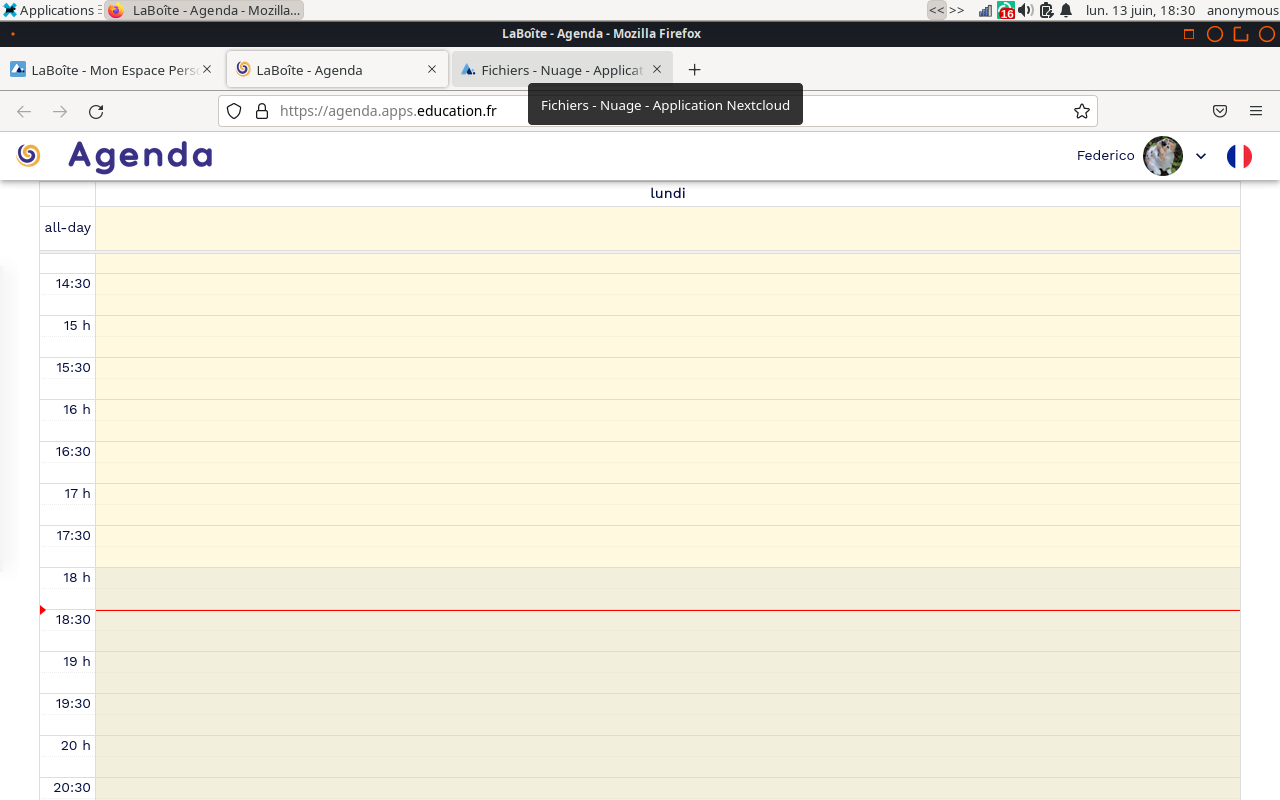
\includegraphics{Captures/agenda.jour.png}
\end{figure}

\begin{figure}
    \centering
    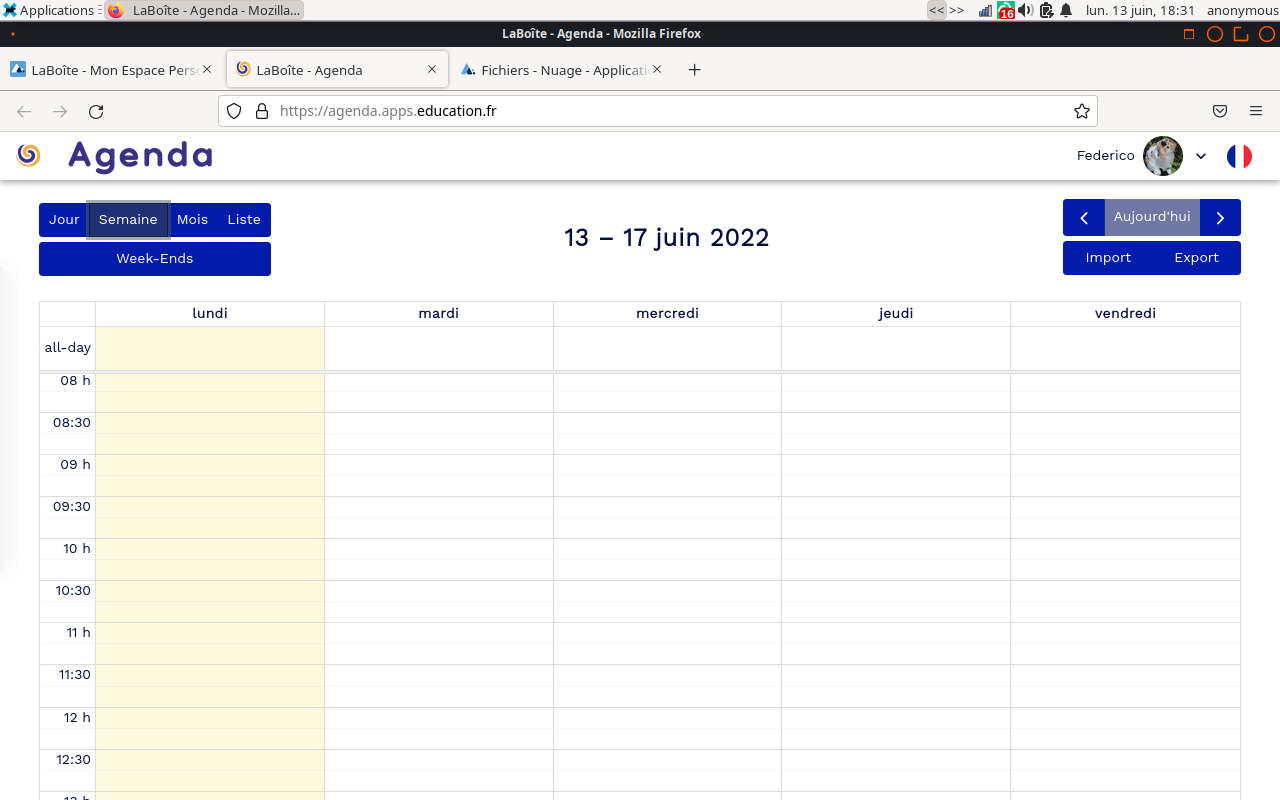
\includegraphics{Captures/agenda.semaine.png}
\end{figure}

\begin{figure}
    \centering
    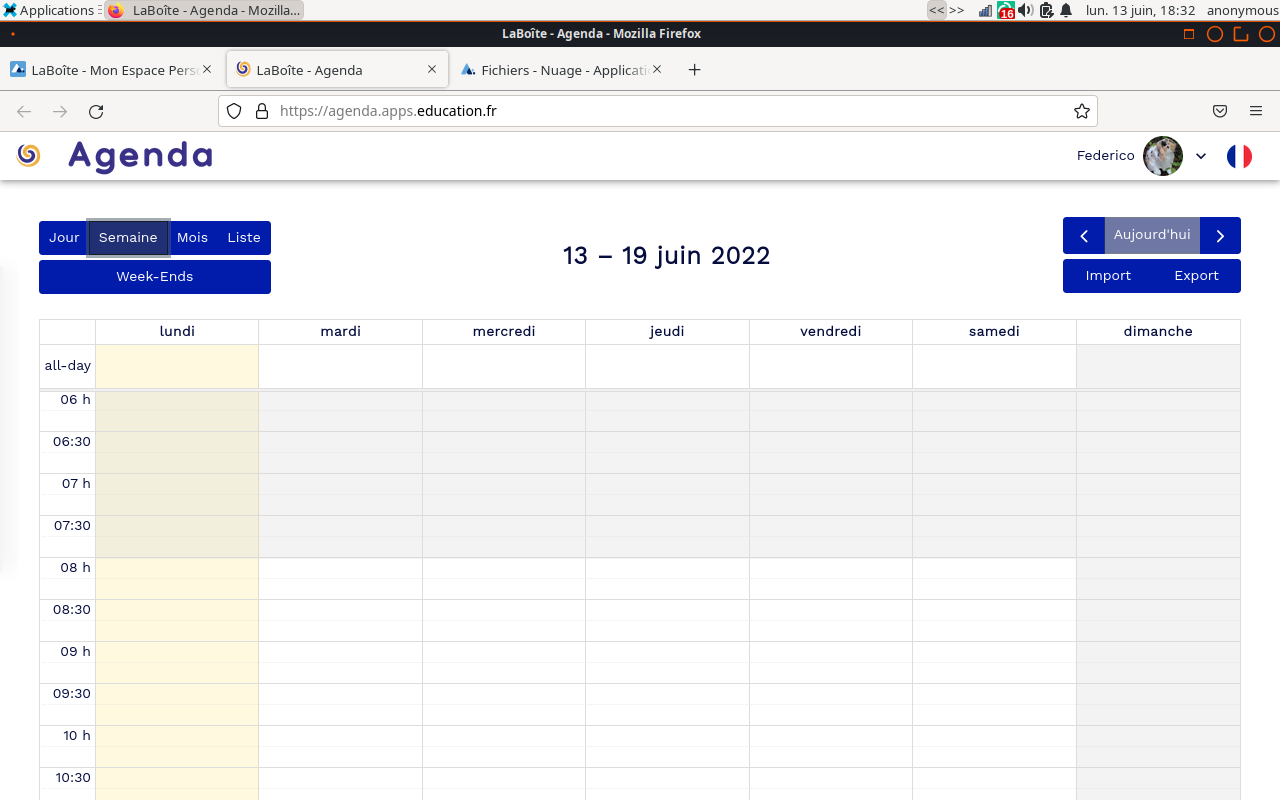
\includegraphics{Captures/agenda.semaine.we.png}
\end{figure}

%\begin{figure}
%    \centering
%    \includegraphics{}
%\end{figure}

%\begin{figure}
%    \centering
%    \includegraphics{}
%\end{figure}

%\begin{figure}
%    \centering
%    \includegraphics{}
%\end{figure}

\newpage
\renewcommand{\baselinestretch}{1}
\setlength{\parskip}{0em}
\tableofcontents

\end{document}